% !TeX root = ../../../main.tex

\begin{figure}
	\centering
	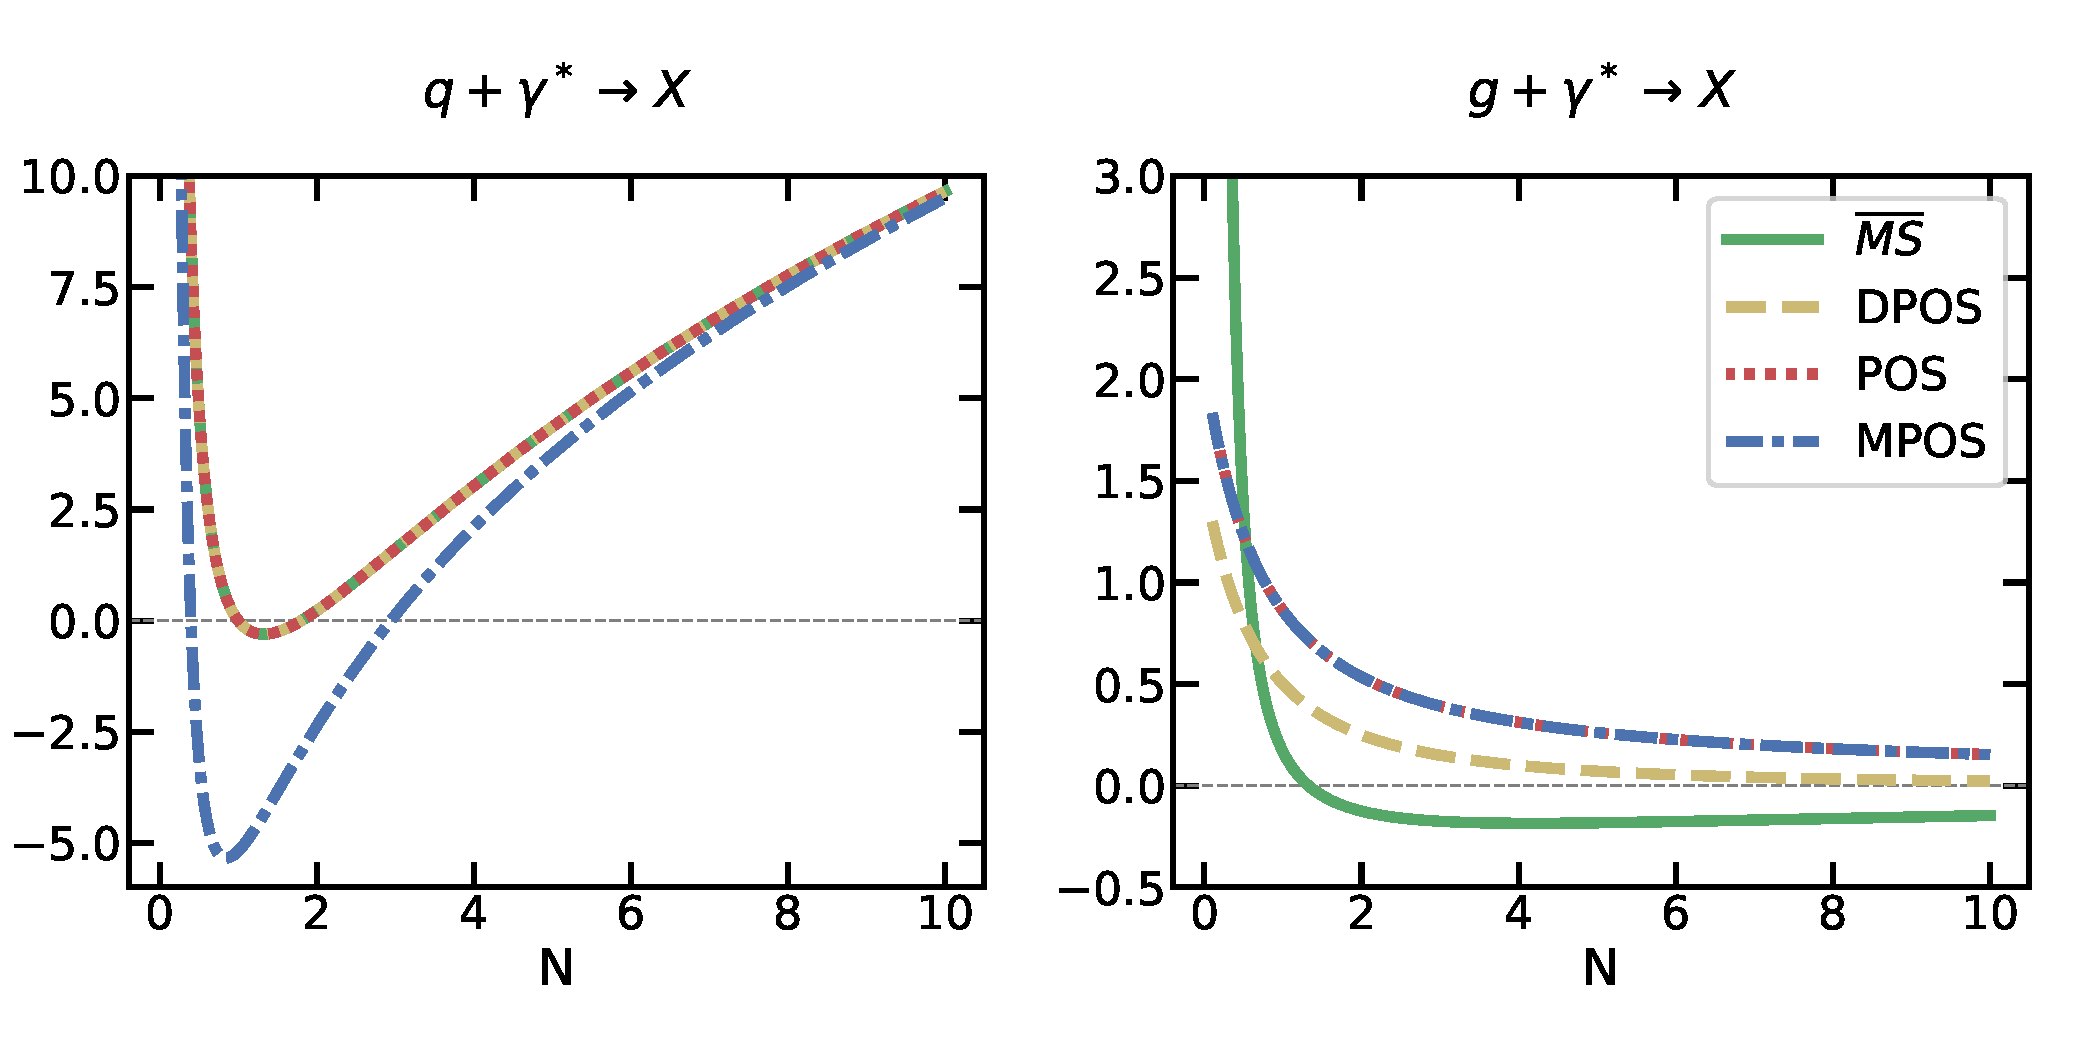
\includegraphics[width=0.6\textwidth]{ch-qcd/dis}
	\caption{
		The \lo Feynman diagram associated to the scattering of a lepton (electron
		in picture) against an hadron component, mediated by an \ew boson.
	}
	\label{fig:qcd/dis}
\end{figure}


The Deep Inelastic Scattering process is the scattering of a lepton over an
hadron component, mediated by an \ew boson \cref{fig:qcd/dis}\footnote{
	This and the other Feynman diagrams in this chapter are taken from the
	\href{https://wiki.physik.uzh.ch/cms/latex:feynman}{related CMS wiki page
		of the Zurich University}.
}.
%
Since the scattering happens directly on a constituent of the incoming hadron,
isolating it from the composite particle (and thus destroying the latter), it
is called \textit{deep inelastic}.
%
The leptonic part does not couple directly to \qcd , thus the $\alpha_s$
corrections do apply only to the hadronic side (at \lo \ew), and the \ew boson
can be seen as emitted from the incoming lepton and absorbed into the hadron.
%
In this picture the process can be interpreted as the scattering of an
off-shell \ew boson over an hadron, probing the hadron composition.

As discussed in the former section, the history of the \dis process is deeply
connected to the parton model before, and \pdfs determination afterwards,
since data from several \dis experiments has been used to provide the main
constraints on the \pdfs.
%
Multiple old and more recent \dis experiments are still giving a relevant
contribution to modern datasets used to extract \pdfs, including:
\acrfull{slac}, \acrfull{bcdms}, \acrfull{chorus}, \acrfull{nmc}, and the more
recent \nutev.
%
But the \dis data that mostly constrained \pdfs have been the results from
\hone and \zeus experiments at \hera.

The entire \cref{ch:dis} will be dedicated to the review of the theory
predictions for this process, and to present a software package, \yadism,
dedicated to the calculation of them, with all relevant variants and options.
